\documentclass{beamer}
\usetheme{Madrid}
\usepackage{array}  % Pour des options de tableau avancées
\usepackage{booktabs}  % Pour des lignes de tableau plus jolies
\usepackage{multirow}  % Pour les cellules fusionnées
\usepackage[table,xcdraw]{xcolor}  % Pour les couleurs de tableau
\usepackage{graphicx}  % Pour redimensionner les tableaux et insérer des images

% Définir une nouvelle couleur
\definecolor{mycolor}{RGB}{0, 128, 0}  % Vert foncé par exemple

% Appliquer la nouvelle couleur aux éléments souhaités
\setbeamercolor{structure}{fg=mycolor}  % Change la couleur des titres et des sections

\title{Stage Laboratoire E3S}
\author{Kossi ABOTSI}
\date{\today}

\begin{document}
	\begin{frame}[plain]
		\maketitle
	\end{frame}
	\begin{frame}{Introduction}
		La question de recherche est d'examiner les conditions qui augmentent ou diminuent les différences entre les sexes dans l'engagement dans l'activité physique pendant les cours d'éducation physique, dans le cadre écologique.
	\end{frame}
	\begin{frame}{Objectif}
		 Notre objectif dans ce stage est d'examiner les écarts de MVPA (moderate to vigorous physical activity) des filles et garçons mesurés au cours d'une leçon d'EPS de 2h au regard de quatres variables : le sexe, la nature de l'activité (CA = champ d'apprentissage), la catégorie socioculturelle de l'établissement (catégorie d'IPS = indice de position sociale) et la catégorie socioprofessionnelle des parents (CSP).
	\end{frame}
	
	\begin{frame}{Données}
		Pour atteindre nos objectifs, nous disposons de mesures de MVPA des élèves de différentes classes dont nous connaissons aussi le sexe, la nature de l'activité effectuée, la catégorie socioculturelle de l'établissement et la catégorie socioprofessionnelle du père et de la mère. Au total on a notre disposition 462 observations.\\
	\end{frame}
	\begin{frame}{Questions à répondre et Modèle à utiliser}
		\begin{itemize}
			\item Les écarts de MVPA entre filles et garçons selon les CA (CA1, CA2, CA3, CA4).
			\item Les écarts de MVPA entre filles et garçons selon la catégorie d’IPS du collège (élevé, moyen, faible).
			\item Les écarts de MVPA entre filles et garçons selon le milieu géographique (urbain, rural).
			\item Les écarts de MVPA entre filles et garçons selon le CSP des parents.
		\end{itemize}
		Dans ces 4 questions, nous voulons expliquer une variable quantitative continue en fonction de deux variables qualitatives. Donc le modèle statistique adapté est une ANOVA à deux facteurs avec interaction.
	\end{frame}
	
	\begin{frame}{Les écarts de MVPA entre filles et garçons selon les CA (CA1, CA2, CA3, CA4) Partie 1}
		ANOVA à deux facteurs :   
		\begin{itemize}
			\item Variables dépendantes : écart de MVPA de chaque élève à la moyenne de sa classe
			\item Variables indépendantes qualitatives : genre, CA et interaction entre genre et CA
		\end{itemize}
		\textbf{Les hypothèses de normalité et d'homoscédasticité des résidus du modèle étant vérifiées, on peut regarder les résultats.}
	\end{frame}
	\begin{frame}{Résultats de l'ANOVA}
		\textbf{Significativité de l'effet de l'interaction}
		\begin{table}[h!]
			\centering
			\resizebox{\textwidth}{!}{%
				\begin{tabular}{|>{\raggedright\arraybackslash}m{5cm}|>{\centering\arraybackslash}m{2cm}|>{\centering\arraybackslash}m{2cm}|>{\centering\arraybackslash}m{2cm}|>{\centering\arraybackslash}m{2cm}|}
					\hline
					& \textbf{CA1} & \textbf{CA2} & \textbf{CA3} & \textbf{CA4} \\
					\hline
					\textbf{Écart entre fille et garçon des écarts à la moyenne de MVPA dans chaque classe} & -4.4548 & -1.4898 & -1.7470 & -9.7647 \\
					\hline
					\textbf{Intervalle de confiance} & -12.010 à 3.100 & -6.4730 à 3.493 & -6.759 à 3.265 & -13.286 à -6.244 \\
					\hline
					\textbf{P-valeur} & 0.6235 & 0.9850 & 0.96 & 0.000 \\
					\hline
			\end{tabular}}
			\caption{Tableau des écarts, intervalles de confiance et p-valeurs pour chaque classe (CA1 à CA4)}
			\label{tab:resultats}
		\end{table}
	\end{frame}
	\begin{frame}{Les écarts de MVPA entre filles et garçons selon les CA (CA1, CA2, CA3, CA4) Partie 2}
		\begin{figure}
			\centering
			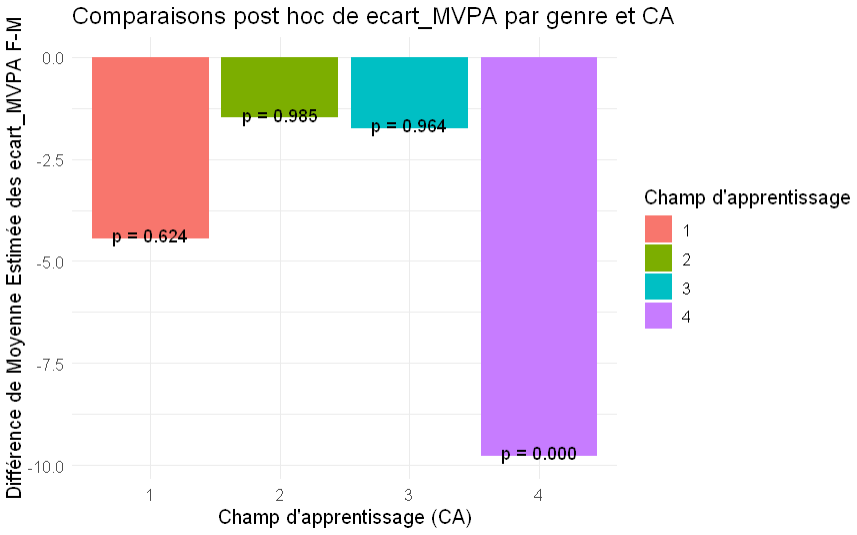
\includegraphics[width=\textwidth]{res_2.PNG}
			\caption{Comparaisons post hoc de l'écart\_MVPA par genre et CA}
		\end{figure}
	\end{frame}
	
	\begin{frame}{Les écarts de MVPA entre filles et garçons selon les CA (CA1, CA2, CA3, CA4) Partie 3 : Taille d'effets}
		\begin{table}[h!]
			\centering
			\resizebox{\textwidth}{!}{%
				\begin{tabular}{|c|c|c|}
					\hline
					\textbf{Parameter} & \textbf{Omega2 (partial)} & \textbf{95\% CI} \\
					\hline
					gender & 0.05 & [0.02, 1.00] \\
					\hline
					CA & 0.00 & [0.00, 1.00] \\
					\hline
					gender:CA & 0.05 & [0.02, 1.00] \\
					\hline
				\end{tabular}
			}
			\caption{Omega2 (partial) avec intervalle de confiance}
		\end{table}
		
		\begin{itemize}
			\item La taille d'effet pour le facteur genre est 0.05, ce qui signifie que 5\% de la variance totale de la variable dépendante (écart\_MVPA) peut être attribuée à l'effet du genre.
			\item La taille d'effet pour l'interaction entre genre et CA est 0.05, ce qui signifie que 5\% de la variance totale de la variable dépendante (écart\_MVPA) peut être attribuée à l'effet de l'interaction.
			\item La taille d'effet pour le facteur CA est 0, ce qui signifie que 0\% de la variance totale de la variable dépendante (écart\_MVPA) peut être attribuée à l'effet du CA.
		\end{itemize}
	\end{frame}
	
	\begin{frame}{Les écarts de MVPA entre filles et garçons selon la catégorie d’IPS du collège (élevé, moyen, faible)}
		ANOVA à deux facteurs : 
		\begin{itemize}
			\item Variables dépendantes : écart de MVPA de chaque élève à la moyenne de sa classe.
			\item Variables indépendantes qualitatives : genre, catégorie d'IPS du collège et interaction entre genre et catégorie d'IPS.
		\end{itemize}
		\textbf{Les hypothèses de normalité et d'homoscédasticité des résidus du modèle étant vérifiées, on peut regarder les résultats.}
	\end{frame}
	\begin{frame}{Résultat de l'ANOVA}
		\begin{itemize}
			\item Interaction non significative.
			\item La catégorie d'IPS du collège n'est pas également significative.
		\end{itemize}
			\begin{table}[h!]
			\centering
			\resizebox{\textwidth}{!}{%
				\begin{tabular}{|>{\raggedright\arraybackslash}m{5cm}|>{\centering\arraybackslash}m{3cm}|>{\centering\arraybackslash}m{3cm}|>{\centering\arraybackslash}m{3cm}|}
					\hline
					& \textbf{Faible} & \textbf{Moyen} & \textbf{Élevé} \\
					\hline
					\textbf{Écart entre fille et garçon des écarts à la moyenne de MVPA de chaque classe} & -5.57 & -5.57 & -5.57 \\
					\hline
					\textbf{Intervalle de confiance} & -7.13 à -4.01 & -7.13 à -4.01 & -7.13 à -4.01 \\
					\hline
					\textbf{P-valeur} & 0.000 & 0.000 & 0.000 \\
					\hline
				\end{tabular}
			}
			\caption{Tableau des écarts, intervalles de confiance et p-valeurs selon la catégorie d'IPS}
			\label{tab:resultats_ips}
		\end{table}
		
		Donc l'IPS\_categorie n'a aucune influence sur les écarts de MVPA à la moyenne de chaque classe des filles et garçons et aussi dans toutes ces catégories les garçons ont les écarts à la moyenne de mvpa significativement supérieur à celui des filles.
	\end{frame}
	
	\begin{frame}{Les écarts de MVPA entre filles et garçons selon le milieu géographique (urbain, rural) Partie 1}
		ANOVA à deux facteurs :   
		\begin{itemize}
			\item Variables dépendantes : écart de MVPA de chaque élève à la moyenne de sa classe.
			\item Variables indépendantes qualitatives : genre, milieu géographique et interaction entre genre et milieu géographique.
		\end{itemize}
		\textbf{Les hypothèses de normalité et d'homoscédasticité des résidus du modèle étant vérifiées, on peut regarder les résultats.}
	\end{frame}
	\begin{frame}{Résultats de l'ANOVA}
		\textbf{Significativité de l'effet de l'interaction}
		\begin{table}[h!]
			\centering
			\resizebox{\textwidth}{!}{%
				\begin{tabular}{|>{\raggedright\arraybackslash}m{5cm}|>{\centering\arraybackslash}m{2.5cm}|>{\centering\arraybackslash}m{2.5cm}|}
					\hline
					& \textbf{Rural} & \textbf{Urbain} \\
					\hline
					\textbf{Écart entre fille et garçon des écarts à la moyenne de MVPA de chaque classe} & -2.44 & -8.06 \\
					\hline
					\textbf{Intervalle de confiance} & -5.49 à 0.602 & -10.761 à -5.350 \\
					\hline
					\textbf{P-valeur} & 0.1650 & 0.000 \\
					\hline
			\end{tabular}}
			\caption{Tableau des écarts, intervalles de confiance et p-valeurs selon le milieu géographique}
			\label{tab:resultats_geographique}
		\end{table}
	\end{frame}
	
	\begin{frame}{Les écarts de MVPA entre filles et garçons selon le milieu géographique (urbain, rural) Partie 2}
		\begin{figure}
			\centering
			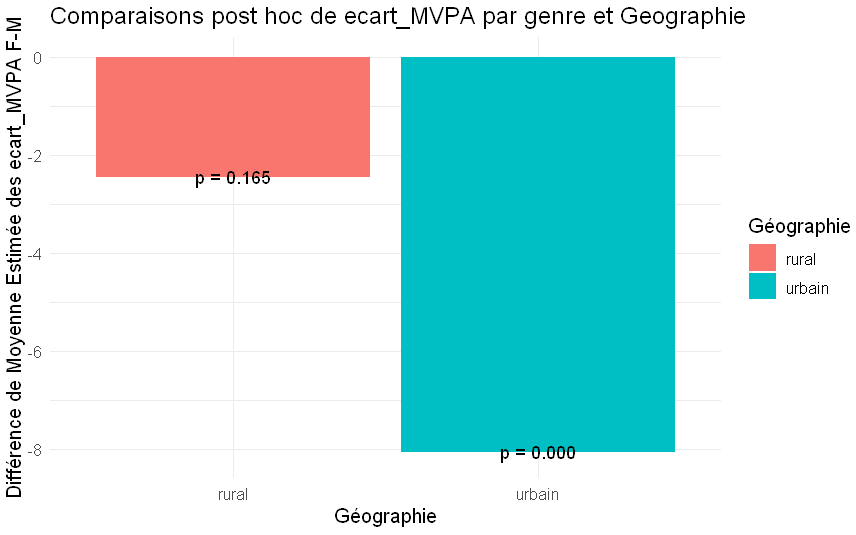
\includegraphics[width=\textwidth]{res_3.PNG}
			\caption{Comparaisons post hoc de l'écart\_MVPA par genre et CA}
		\end{figure}
	\end{frame}
	\begin{frame}{Les écarts de MVPA entre filles et garçons selon le milieu géographique (urbain, rural) Partie 3}
		\begin{table}[h!]
			\centering
			\resizebox{\textwidth}{!}{%
				\begin{tabular}{|>{\raggedright\arraybackslash}m{5cm}|>{\centering\arraybackslash}m{3cm}|>{\centering\arraybackslash}m{4cm}|}
					\hline
					& \textbf{Omega2 (partial)} & \textbf{95\% CI} \\
					\hline
					\textbf{gender} & 0.09 & [0.05, 1.00] \\
					\hline
					\textbf{Geographie} & 0.00 & [0.00, 1.00] \\
					\hline
					\textbf{gender:Geographie} & 0.02 & [0.01, 1.00] \\
					\hline
			\end{tabular}}
			\caption{Tableau des Omega2 (partial) et intervalles de confiance pour chaque paramètre}
		\end{table}
		\begin{itemize}
			\item La taille d'effet pour le facteur gender est 0.09 ce qui signifie que 9\% de la variance totale de la variable dépendante (écart\_MVPA) peut être attribuée à l'effet du genre.
			\item La taille d'effet pour l'interaction entre genre et Geographie est 0.02 ce qui signifie que 2\% de la variance totale de la variable dépendante (écart\_MVPA) peut être attribuée à l'effet de l'interaction.
		\end{itemize}
	\end{frame}
\end{document}
